\section{Elecció de les condicions de disseny}
Donada l'alçada i la velocitat de vol, així com $T_{t4}$ les tres variables necessàries per fer el disseny són $\pi_c$, $\pi_f$ i $\alpha$. Aquests s'han d'escollir per tal d'obtenir el millor motor possible donades les dades de l'enunciat mostrades a l'apartat \ref{descripcio}.
La definició dels paràmetres de disseny es:
\begin{equation*}
	\pi_c = \frac{P_{3t}}{P_{2t}} = \pi_{f}\times\pi_{cL} = \frac{P_{2.5t}}{P_{2t}} \times \frac{P_{3t}}{P_{2.5t}}
\end{equation*}
\begin{equation*}
	\pi_f = \frac{P_{2.5t}}{P_{2t}} = \frac{P_{1.3t}}{P_{2t}} 
\end{equation*}
\begin{equation*}
	\alpha = \frac{m_{primari}}{m_{secundari}}
\end{equation*}
\noindent Per fer la tria,  s'ha fet un extens estudi amb l'objectiu de trobar els paràmetres adequats a les condicions de vol proporcionades a l'enunciat i als criteris de disseny imposats. Aquests es troben integrat a la funció \textit{opt\_parametros.m}, que prova diferents combinacions de $\pi_f$ i $\pi_c$ i calcula amb elles la força adimensional. Es busca maximitzar aquest paràmetre per poder obtenir un motor petit. Tal i com es veu a la Figura \ref{Fadimensional}, al incrementar $\pi_f$ i $\pi_c$ també incrementa \(\hat{F}\) i no es possible calcular cap màxim. S'adopta la idea de que, quan al augmentar els valors de $\pi_f$ i $\pi_c$, \(\hat{F}\) no incrementa més d'un 5\% no val la pena continuar augmentant els ratis de compressió.
\begin{figure}[H]
	\centering
	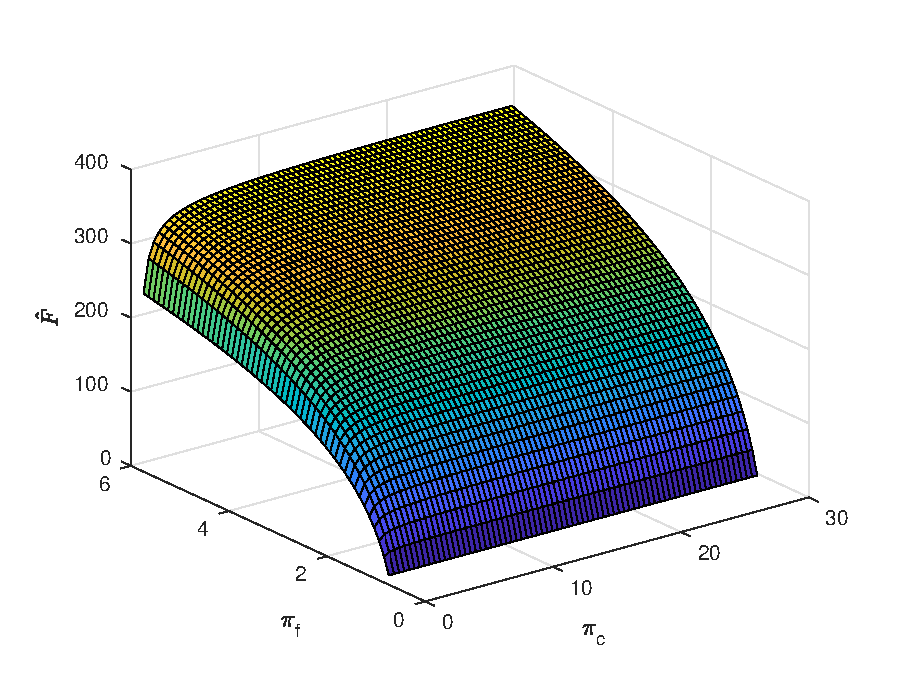
\includegraphics[width=0.35\textwidth]{./pics/F_pc_pf}
	\caption{\(\hat{F}\) en funció de $\pi_c$ i $\pi_f$}
	\label{Fadimensional}
\end{figure}
A més de maximitzar la força adimensional, es vol garantir un consum específic mínim. Per cada combinació  $\pi_f$ i $\pi_c$ de valors, es pot obtenir la $\alpha$ corresponent per complir aquest requisit, seguint el procediment proposat a \cite[5-10]{mattingly} que principalment es basa en imposar:
\begin{equation*}
	\frac{\partial S}{\partial \alpha} = 0 
\end{equation*}
Arribant així a:
\begin{multline}
	\alpha_{opt} = \frac{1}{\tau_r(\tau_f-1)}\bigg[\tau_{\lambda}-\tau_r(\tau_c-1)-\frac{\tau_{\lambda}}{\tau_r\tau_c} \\ -\frac{1}{4}(\sqrt{\tau_r\tau_f-1} + \sqrt{\tau_r-1})^2\bigg]
\end{multline}
\begin{figure}[H]
	\centering
	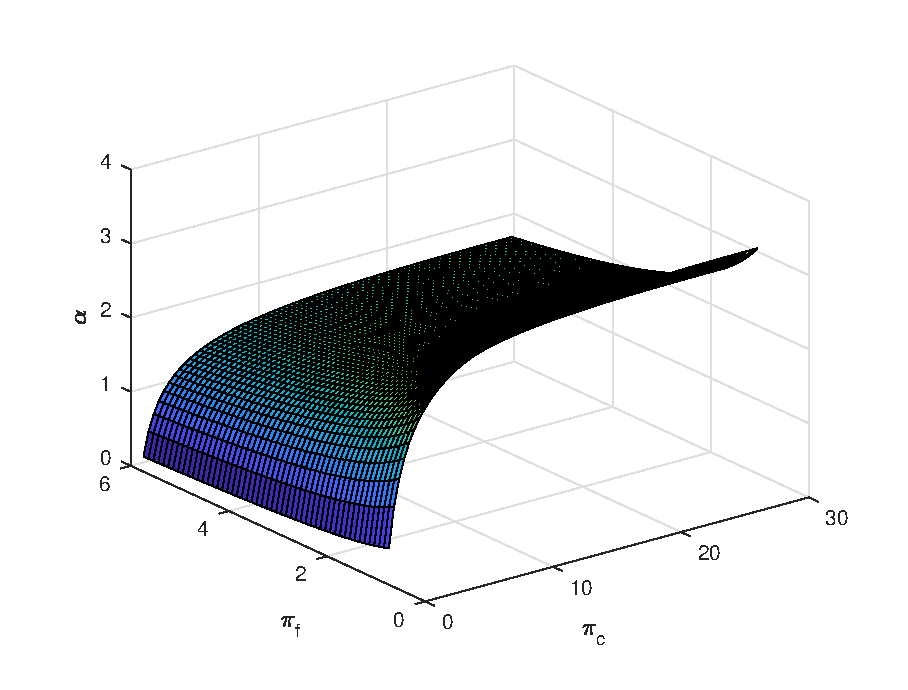
\includegraphics[width=0.35\textwidth]{./pics/alpha_pc_pf}
	\caption{$\alpha_{opt}$ en funció de $\pi_c$ i $\pi_f$}
\end{figure}
Finalment, els valors obtinguts són els següents:
\begin{figure}[H]
	\centering
	\begin{tabular}{lc}
		\toprule[3pt]
		\textbf{Paràmetre}&\textbf{Valor}\\
		\midrule[1pt]
		$\pi_{c}$ & 22.60 \\
		$\pi_{f}$ & 2.20 \\
		$\alpha_{opt}$ & 2.35 \\
		\bottomrule[2pt]
	\end{tabular}
	\label{C_opti2}
	\caption{Selecció dels paràmetres de disseny}
\end{figure}
\noindent Aquests s'han comparat a valors típics d'altres aeronaus i s'ha conclòs que són uns valors raonables i realistes. Tot el procés realitzat es pot veure esquematitzat a la Figura \ref{opt}.
Resumidament, s'ha anat variant $\pi_c$ o $\pi_f$ fins arribar a una convergència de valors que donés un increment no significatiu de $\hat{F}$. 
\begin{figure}[H]
	\centering
	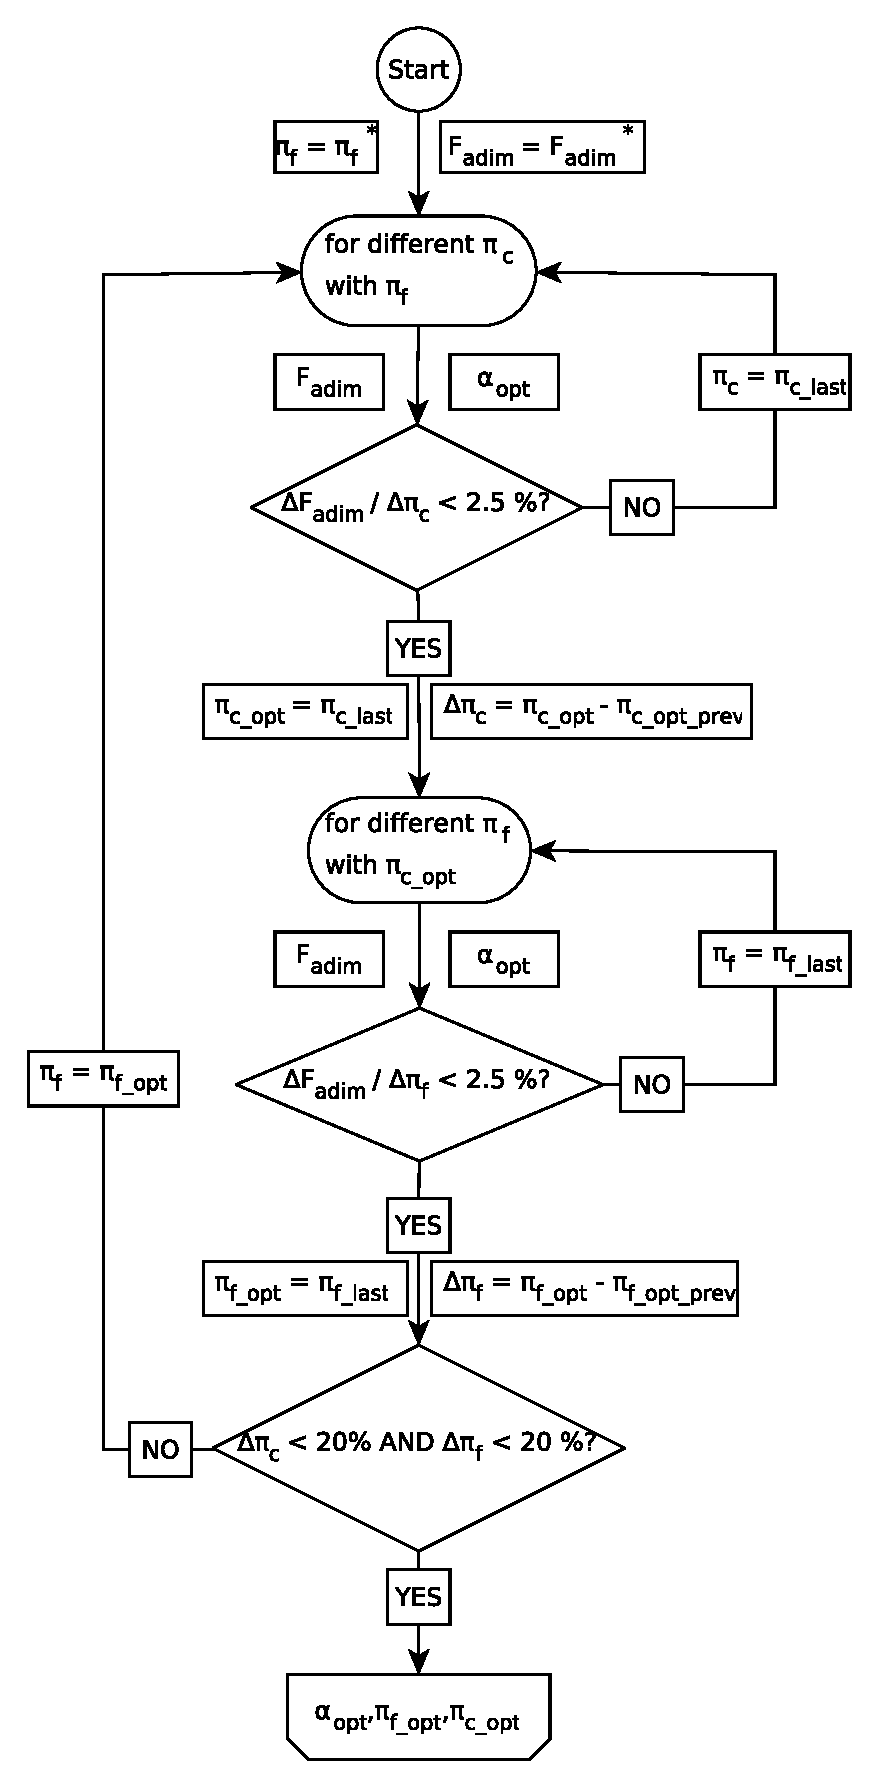
\includegraphics[scale=0.6]{./pics/optimization}
	\caption{Algoritme emprat per trobar els valors òptims}
	\label{opt}
\end{figure}
\section{Càlcul paramètric del motor real}
El següent pas consisteix a resoldre el turbofan real sencer, sense tindre en compte \textit{mixer} ni \textit{afterburner}, obtenint així la distribució de pressions, temperatures i fluxos màssics. A continuació es mostren algunes consideracions rellevants per a cada etapa \footnote{La I indica ideal mentre que la R, real.}:
\begin{itemize}
\item \textbf{0t - 2t: Difusor}. Es considera adiabàtic i per tant, $\tau_d = 1$. Per altra banda si que es produeix una pèrdua de pressió total que es manifesta com $\pi_d = \eta_d$.
\item \textbf{2t - 2.5t: Fan}. Com que la tasca primordial del fan es incrementar la pressió, es fixa la pressió que assoleix el compressor ideal i es dissenya el cas real per tal que assoleixi el mateix objectiu, es a dir, la pressió de sortida es manté constant però la temperatura varia segons la eficiència. Així, $P_{t25}^R = P_{t25}^I$ tot i que $T_{t25}^R \neq T_{t25}^I$ . Coneixent el rendiment $\eta_f$ es troben les noves temperatures.
\item \textbf{2.5t - 3t: Compressor de baixa}. La mateixa explicació del fan és vàlida per al compressor de baixa doncs es dissenya amb el mateix criteri.
\item \textbf{3t - 4t: Cambra de combustió}. En un cas ideal la combustió es produeix de forma isòbara mentre que al cas real hi ha una pèrdua de pressió total. Ds dissenya per tal d'arribar a la $T_{t4}$ de disseny. El consum de combustible es troba igualant la calor generada per la crema a la calor proporcionada al fluid. Es important esmentar que en la realització del codi no s'han fet simplificacions com considerar $C_P=ct$ o $(1+f)\simeq1$.
\item \textbf{4t - 4.5t: Turbina d'alta}. L'objectiu de la tovera real serà el d'aconseguir expandir el fluid per tal d'aportar el treball necessari al compressor. Per resoldre la turbina doncs, cal igualar treballs. Concretament: $\dot{W_{cH}^R} = \dot{W_{tH}^R} $. D'aquesta igualtat s'obté $\tau_{tH}^R$ que si es combina amb $\eta_{tH}$ s'obté $\tau_{tH}^I$ que permet trobar  $P_{tH}^{I} = P_{tH}^{R}$.
\item \textbf{4.5t - 6t: Turbina de baixa}. La mateixa explicació de la turbina d'alta serveix per la de baixa, amb la diferència que ara el treball s'iguala al del fan.
\item \textbf{6t - 9t: Tovera Primari}. Es considera adiabàtica i per tant, $\tau_n = 1$. Per altra banda, $\pi_n = \eta_n$. Per últim, per trobar els valors dinàmics a la sortida, es suposa que la tovera està adaptada ($P_9 = P_0$) i si no ho està es restringeix el valor $M_9=1$ ja que considerem tovera convergent.
\item \textbf{16t - 19t: Tovera Secundari}. Funciona exactament igual que la del primari però amb les condicions d'entrada del flux secundari.
\end{itemize}
Finalment, els resultats obtinguts que dóna el programa \textbf{MAIN\_TURBOFAN.m} amb les opcions de \textit{mixer}, \textit{afterburner} i \textit{propeller} desactivades són:
\begin{table}[H]
\centering
\begin{tabular}{lcccc}
\toprule[3pt]
\textbf{Etapa} &\textbf{$\bm{\pi}$} & \textbf{$\bm{\tau}$}    & \textbf{Pt} [kPa]  & \textbf{Tt} [K]  \\
\midrule[1pt]
0 - 0t     & 1.23   & 1.06  & 35.10   & 240.22             \\
0t - 2t     & 0.96   & 1  & 33.70   & 240.22             \\
2t - 2.5t/13t     & 2.20   & 1.29  & 74.13   & 309.20             \\
2.5t - 3t     & 10.27  & 2.07  & 761.52   & 641.44             \\
3t - 4t     & 0.94     & 0.76  & 715.83  & 1780.00             \\
4t - 4.5t     & 0.43   & 0.85  & 311.23   & 1509.20             \\
4.5t - 6t     & 0.51   & 0.88  & 159.00   & 1320.70             \\
6t - 9t     & 0.98   & 0.92  & 155.81   & 1320.70            \\
16t - 19t     & 0.98   & 0.92  & 72.65   & 309.20            \\
\bottomrule[2pt]
\end{tabular}
\caption{Pressions i Temperatures - motor real}
\end{table}
Pel que fa als fluxos màssics:
\begin{figure}[H]
	\centering
	\begin{tabular}{lc}
		\toprule[3pt]
		\textbf{Paràmetre}&\textbf{Valor [kg/s]}\\
		\midrule[1pt]
		$m_{o}$ & 15.06 \\
		$m_{sec}$ & 35.46 \\
		$m_{f}$ & 0.56 \\
		\bottomrule[2pt]
	\end{tabular}
	\label{C_opti2}
	\caption{Fluxos màssics - motor real}
\end{figure}
Per aquesta configuració s'obté una empenta adimensonal de $\bm{\hat{F} = 5.5}$.